\documentclass[crop,tikz,border=0.1cm]{standalone}

% math and formulas
\usepackage{amsmath}
\usepackage{amsfonts}
\usepackage{amssymb}
\usepackage[amssymb]{SIunits}
\usepackage{mathtools}
\usepackage{esvect} % for vector typesetting
\usepackage{bm} % for matrix typesetting
\usepackage{xfrac}

\usepackage{environ}


% ---Notation macros---

% math
\let\oldvec\vec
% \renewcommand{\vec}[1]{\bm{\mathbf{#1}}}
\renewcommand{\vec}[1]{\bm{#1}} % \bm vs \mathbf
\newcommand{\vecf}[1]{\bm{#1}} % \bm vs \mathbf
\newcommand{\vecelem}[1]{#1}
\newcommand{\vecarrow}[1]{\vv{#1}}
\newcommand{\mat}[1]{\bm{#1}}
\newcommand{\matelem}[1]{\mathit{#1}}
\newcommand{\ten}[1]{\mathbf{#1}}
\newcommand{\tenelem}[1]{\mathrm{#1}}
\newcommand{\set}[1]{\mathbb{#1}}

\newcommand{\trans}[1]{#1^{\mathsf{T}}}
\newcommand{\ifrac}[2]{\sfrac{#1}{#2}}
\newcommand{\deriv}[2]{\frac{\text{d}#1}{\text{d}#2}}
\newcommand{\partderiv}[2]{\frac{\partial #1}{\partial #2}}
\newcommand{\ideriv}[2]{\ifrac{\text{d}#1}{\text{d}#2}}
\newcommand{\ipartderiv}[2]{\ifrac{\partial #1}{\partial #2}}

\DeclarePairedDelimiter{\norm}{\lVert}{\rVert}

% machine learning
\newcommand{\param}{\lambda}


% misc
\newcommand{\keyword}[1]{\textbf{#1}}
\newcommand{\para}{\par\medskip}
\newcommand{\ds}{\displaystyle}

\newcommand{\keycode}[1]{\texttt{#1}}
\newcommand{\code}[1]{\texttt{#1}}


\let\oldcite\cite
\renewcommand{\cite}[1]{{\color{red}(\oldcite{#1})}\\}



% --- TIKZ ---

\NewEnviron{defbox}[1]
{
  \centering

  \tikzstyle{mybox} = [draw=red, fill=blue!40!pagecolor, very thick, rectangle, rounded corners, inner sep=10pt, inner ysep=20pt]
  \tikzstyle{fancytitle} = [fill=red, text=white]
  \begin{tikzpicture}
    \node [mybox] (box) {%
      \begin{minipage}{1.0\textwidth}
        \BODY
      \end{minipage}
    };
    \node [right,inner xsep=1em,fill=red!75, text=white,outer sep=0pt,text height=2ex,text depth=.5ex] (title)
    at ([shift={(-1em,0pt)}]box.north west) {#1};
    \fill[red!50!black] (title.north east) -- +(-1em,1em) -- +(-1em,0) -- cycle;
    \fill[red!50!black] (title.south west) -- +(1em,-1em) -- +(1em,0) -- cycle;

  \end{tikzpicture}
}


\NewEnviron{infobox}[1]
{
  \centering

  \tikzstyle{mybox} = [draw=blue, fill=green!40!pagecolor, very thick, rectangle, rounded corners, inner sep=10pt, inner ysep=20pt]
  \tikzstyle{fancytitle} = [fill=blue, text=white]
  \begin{tikzpicture}
    \node [mybox] (box) {%
      \begin{minipage}{1.0\textwidth}
        \BODY
      \end{minipage}
    };
    \node [right,inner xsep=1em,fill=blue!75, text=white,outer sep=0pt,text height=2ex,text depth=.5ex] (title)
    at ([shift={(-1em,0pt)}]box.north west) {#1};
    \fill[blue!50!black] (title.north east) -- +(-1em,1em) -- +(-1em,0) -- cycle;
    \fill[blue!50!black] (title.south west) -- +(1em,-1em) -- +(1em,0) -- cycle;

  \end{tikzpicture}
}


\NewEnviron{examplebox}[1]
{
  \centering

  \tikzstyle{mybox} = [draw=green, fill=yellow!40!pagecolor, very thick, rectangle, rounded corners, inner sep=10pt, inner ysep=20pt]
  \tikzstyle{fancytitle} = [fill=green, text=white]
  \begin{tikzpicture}
    \node [mybox] (box) {%
      \begin{minipage}{1.0\textwidth}
        \BODY
      \end{minipage}
    };
    \node [right,inner xsep=1em,fill=green!75, text=white,outer sep=0pt,text height=2ex,text depth=.5ex] (title)
    at ([shift={(-1em,0pt)}]box.north west) {#1};
    \fill[green!50!black] (title.north east) -- +(-1em,1em) -- +(-1em,0) -- cycle;
    \fill[green!50!black] (title.south west) -- +(1em,-1em) -- +(1em,0) -- cycle;

  \end{tikzpicture}
}

% \newcommand{\code}{\mint[frame=lines,framesep=2mm,baselinestretch=1.2,bgcolor=lightgray,fontsize=\footnotesize,linenos]{python}}

% \newenvironment{codeblock}
% {
%   \begin{minted}[frame=lines,framesep=2mm,baselinestretch=1.2,bgcolor=lightgray,fontsize=\footnotesize,linenos]{python}
% }
% {
% \end{minted}
% }

% conditional compilation
\newif\ifcp
\cptrue % if commented out -> no compilation

% \ifcp
   %% CONDITIONAL CODE
% \fi


%%% Local Variables:
%%% mode: latex
%%% TeX-master: "../main"
%%% End:


\usepackage{xcolor}
\usepackage{tikz}
\usetikzlibrary{external,3d,matrix,chains,positioning,decorations,calc,intersections,shapes,arrows,fadings,patterns,arrows.meta,quotes}
\usepackage{tikz-3dplot}
%\tikzexternalize
\usepackage{tikzpagenodes}
\usepackage{pgfplots}
\pgfplotsset{compat=1.16}

\usepackage{graphicx}
\graphicspath{{../res/}}

\usepackage{pgf-umlsd}
\usepackage{ifthen}

\begin{document}
\colorlet{pagecolor}{white}
\colorlet{textcolor}{black}

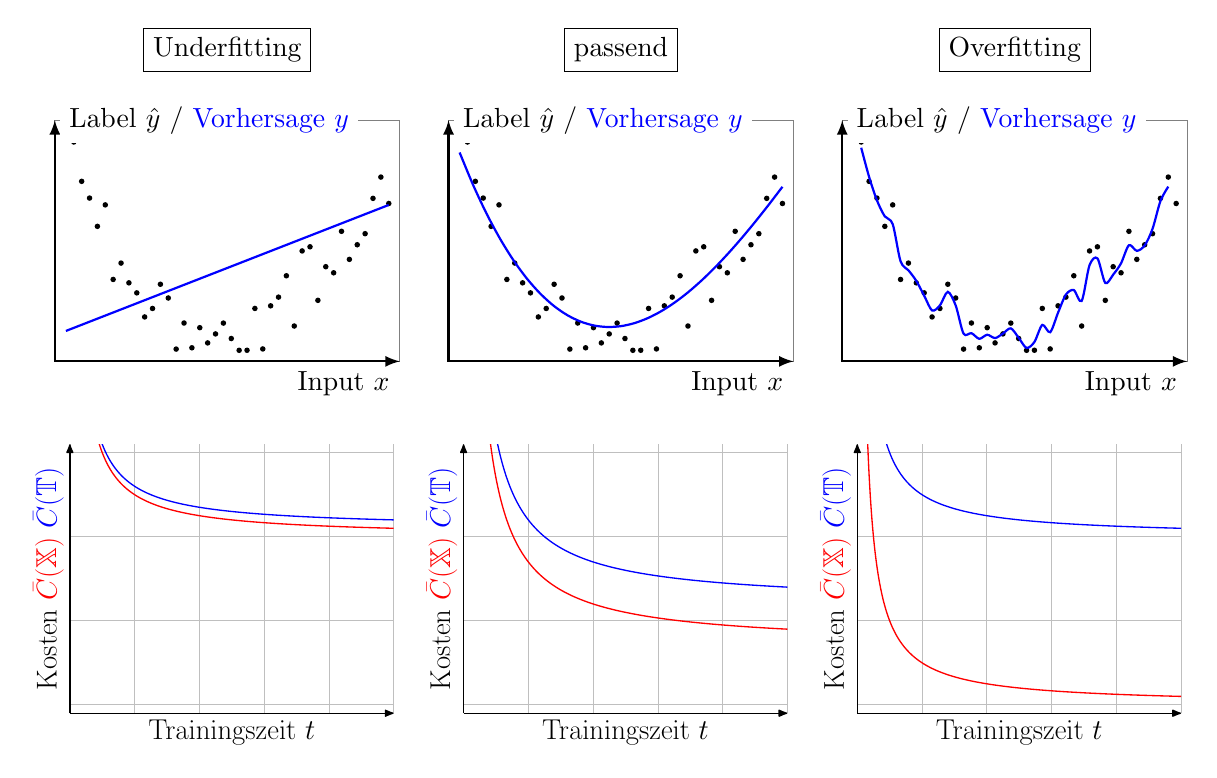
\begin{tikzpicture}[
declare function={f(\x)=0.5*pow(abs(\x-2),2)-0.06*pow(\x-2,3);}]
 \foreach \Z in {1,...,42}
 {\pgfmathsetmacro{\X}{\Z/10}
 \pgfmathsetmacro{\Y}{f(\X)+0.9*rnd}
 \ifnum\Z=1
  \xdef\LstOne{(\X,\Y)}
  \xdef\LstTwo{"(\X,\Y)"}
 \else
  \xdef\LstOne{\LstOne (\X,\Y)}
  \xdef\LstTwo{\LstTwo,"(\X,\Y)"}
 \fi}
%  \begin{scope}[local bounding box=over0]
%  \foreach \Z in {1,...,42}
%  {\pgfmathsetmacro{\Coor}{{\LstTwo}[\Z-1]}
%  \fill \Coor circle[radius=1pt];
%  }
%  \draw plot[smooth] coordinates \LstOne;
%  \end{scope}
 \begin{scope}[local bounding box=over,xshift=-5cm]
 \foreach \Z in {1,...,40}
 {\pgfmathsetmacro{\Last}{{\LstTwo}[\Z-1]}
 \pgfmathsetmacro{\Current}{{\LstTwo}[\Z]}
 \pgfmathsetmacro{\Next}{{\LstTwo}[\Z+1]}
 %\typeout{\Last,\Current,\Next}
  \edef\temp{\noexpand\path ($0.6*\Current+0.2*\Last+0.2*\Next$)   coordinate
  (p\Z);}
  \temp
  \ifnum\Z=1
  \xdef\LstThree{(p\Z)}
  \else
  \xdef\LstThree{\LstThree (p\Z)}
  \fi
  }
 \foreach \Z in {1,...,42}
 {\pgfmathsetmacro{\Coor}{{\LstTwo}[\Z-1]}
 \fill \Coor circle[radius=1pt];
 }
 \draw[thick,blue] plot[smooth] coordinates \LstThree;
 \end{scope}
 %
 \begin{scope}[local bounding box=good,xshift=-10cm]
 \foreach \Z in {1,...,42}
 {\pgfmathsetmacro{\Coor}{{\LstTwo}[\Z-1]}
 \fill \Coor circle[radius=1pt];
 }
 \draw[thick,blue] plot[smooth,domain=0.1:4.2,variable=\x] (\x,{f(\x)+0.45});
 \end{scope}
 %
 \begin{scope}[local bounding box=under,xshift=-15cm]
 \foreach \Z in {1,...,42}
 {\pgfmathsetmacro{\Coor}{{\LstTwo}[\Z-1]}
 \fill \Coor circle[radius=1pt];
 }
 \draw[thick,blue] (0.1,0.4) -- (4.2,2);
 \end{scope}

 \pgfplotsset{every axis/.append style={
     font = \LARGE
     }}


 \begin{scope}[local bounding box=under_cost,shift={($(under)+(-2cm,-6cm)$)},scale=0.6]
   \begin{axis}[
     grid=major,
     xmin=0, xmax=50, ymin=-0.1, ymax=3.1, domain=0:50,
     xlabel={Trainingszeit $t$}, ylabel={Kosten {\color{red}$\bar{C}(\set{X})$} {\color{blue}$\bar{C}(\set{T})$}},
     ticks=none,
     axis x line=bottom,thick,axis line style={-Latex[round]},
     axis y line=left,thick,axis line style={-Latex[round]},
     scale=1]
     \addplot[thick,red, samples=500, smooth] plot (\x, { 5/\x + 2 } );
     \addplot[thick,blue, samples=500, smooth] plot (\x, { 5/\x + 2.1 } );
   \end{axis}
 \end{scope}

 \begin{scope}[local bounding box=over_cost,shift={($(over)+(-2cm,-6cm)$)},scale=0.6]
   \begin{axis}[
     grid=major,
     xmin=0, xmax=50, ymin=-0.1, ymax=3.1, domain=0:50,
     xlabel={Trainingszeit $t$}, ylabel={Kosten {\color{red}$\bar{C}(\set{X})$} {\color{blue}$\bar{C}(\set{T})$}},
     ticks=none,
     axis x line=bottom,thick,axis line style={-Latex[round]},
     axis y line=left,thick,axis line style={-Latex[round]},
     scale=1]
     \addplot[thick,red, samples=500, smooth] plot (\x, { 5/\x } );
     \addplot[thick,blue, samples=500, smooth] plot (\x, { 5/\x + 2 } );
   \end{axis}
 \end{scope}


 \begin{scope}[local bounding box=good_cost,shift={($(good)+(-2cm,-6cm)$)},scale=0.6]
   \begin{axis}[
     grid=major,
     xmin=0, xmax=50, ymin=-0.1, ymax=3.1, domain=0:50,
     xlabel={Trainingszeit $t$}, ylabel={Kosten {\color{red}$\bar{C}(\set{X})$} {\color{blue}$\bar{C}(\set{T})$}},
     ticks=none,
     axis x line=bottom,thick,axis line style={-Latex[round]},
     axis y line=left,thick,axis line style={-Latex[round]},
     scale=1]
     \addplot[thick,red, samples=500, smooth] plot (\x, { 10/\x  + 0.7} );
     \addplot[thick,blue, samples=500, smooth] plot (\x, { 10/\x + 1.2 } );
   \end{axis}
 \end{scope}

 %
 \foreach \X in {over,good,under}
 {\draw[gray,thin] ([xshift=-3pt,yshift=3pt]\X.north west) rectangle
 ([xshift=3pt,yshift=-3pt]\X.south east);
 \draw[latex-latex,thick] ([xshift=-3pt,yshift=3pt]\X.north west) node[right=1.5pt,fill=white]{Label $\hat{y}$ / \color{blue}Vorhersage $y$}
 |- ([xshift=3pt,yshift=-3pt]\X.south east) node[below left]{Input $x$};}



\node[draw,rectangle] at (under.north)[yshift=1cm] {Underfitting};
\node[draw,rectangle] at (good.north)[yshift=1cm] {passend};
\node[draw,rectangle] at (over.north)[yshift=1cm] {Overfitting};
\end{tikzpicture}
%%% Local Variables:
%%% mode: latex
%%% TeX-master: "../figs"
%%% End:


\end{document}

%%% Local Variables:
%%% TeX-command-extra-options: "--shell-escape"
%%% TeX-master: "./figs"
%%% End: